The system was implemented completely using Python (3.10),
which is one of the most widely known programming languages \cite{developer-survey}.
Multiple libraries exist for Python for implementing a wide variety of tasks.
Using high-level libraries is expected to save development time and the popularity of Python
is expected to make the source-code easily approachable for future programmers.

To minimize the latency in reading the data from the sensors,
the system was designed to use parallelism.
The system implements a producer-consumer pattern,
using the Python build-in Multiprocessing library.

The Multiprocessing library is the best of the python built-in parallelism libraries for the task at hand.
The program is synchronous, hence Asyncio is perhaps a too complex solution \cite{python-asyncio}.
While the Threading library would otherwise be a good solution,
it is not truly concurrent as the Python \gls{gil} locks its thread model to a single process \cite{python-threading}.
Multiprocessing, instead, implements process-level parallelism and is capable of achieving "true" concurrency \cite{python-multiprocessing}.

The structure of the program is presented in Figrure \ref{fig:3-block-diagram} as a block diagram.
The program consists of a Main block and five sub-blocks:
\begin{itemize}
    \item Recorder,
    \item Radar module,
    \item RGB-D module,
    \item Infrared module, and
    \item Microphone module.
\end{itemize}

The aforementioned producer-consumer pattern is implemented with all the different blocks being created as parallel processes.
The Radar, Microphone, Infrared and RGB-D modules fetch data from the sensors, making them producers.
The producers output data to queues which are then read by the Recorder block,
hence the Recorder is a consumer.
The main block is neither a producer or a consumer; rather it is responsible for allocating resources for the sub-blocks,
spawning the sub-block processes (subprocesses), controlling them, providing a user interface and writing the metadata file.

\begin{figure}[h]
    \centering
    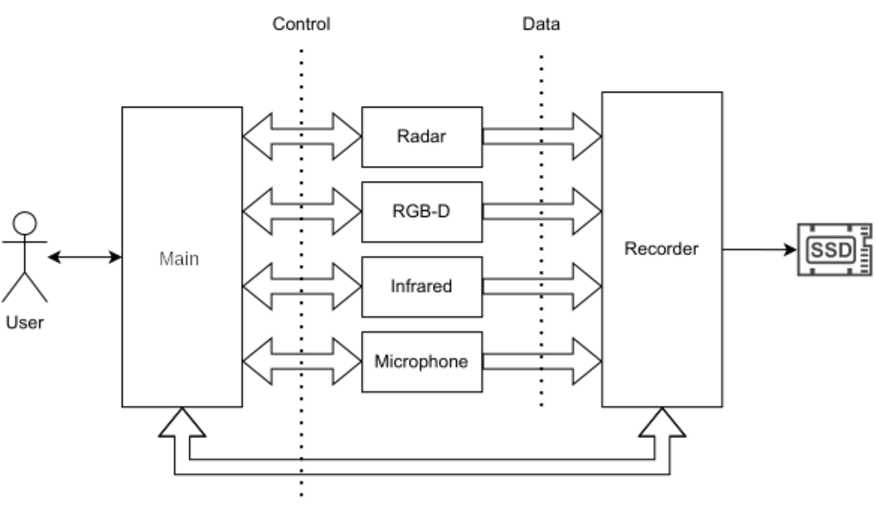
\includegraphics[width=.8\textwidth]{fig/3/block_diagram.pdf}
    \caption{Block diagram of the system.}
    \label{fig:3-block-diagram}
\end{figure}

Inter-process communication is done via \gls{fifo} queues.
Each subprocess is connected to the main process via a single queue.
These queues are colloquially called signaling queues.
In addition, the producers are connected to the Recorder via queues,
one queue per producer. These queues are called the data queues.
The main process creates all these queues and passes them to appropriate subprocesses.

Queues are presented in Figure \ref{fig:3-block-diagram} as single- or double-headed arrows.
A double-headed arrow means that the queue can be written to and read from in both ends,
and single-headed arrow means that data can be read from the pointy end and written from the other.
The signaling queues are read from and written to from both ends,
whereas the data queues are only written to by the producers and read from by the consumer.

While using multiple queues introduces some complexity to the system,
it prevents having to deal with race-conditions.
Another option would have been to use only a single Data queue
and to lock it for writing via mutexes in each of the producers.
The locking operation can block if the mutex is locked from somewhere else,
which could add latency to the data reading operations,
making the multiple queues -approach a better solution.

The control queues are used by the Main process to advance the subprocesses to their next phase.
The subprocesses write to the control queues to indicate their state.
Three kinds of control messages are defined: START, STARTED, and STOP.
The control messages are simply Python String objects with defined content and meaning.
The control messages are documented in Table \ref{tab:control-messages}.

\begin{table}[H]
    \centering
    \begin{tabular}{l l l}
        \toprule
        \textbf{Message} & \textbf{Sender} & \textbf{Meaning} \\
        \midrule
        START & Main & Recipient should start its primary function \\
        STARTED & Producers & Sender has initialized and entered its primary function \\
        STOP & Main & Recipient process should exit \\
        \bottomrule
    \end{tabular}
    \caption{Control messages in the program}
    \label{tab:control-messages}
\end{table}

The flow of the processes consists of three phases: initialization, primary function, and cleanup.
The Main process and the data producers enter the primary function autonomously after the initialization phase is over.
The data producers write the STARTED message to the control queue after this transition.
The Recorder process instead waits for the START message before transitioning from initialization to primary function.
None of the subprocesses enters the cleanup phase autonomously.
They all wait for the Main process to write the STOP message to the control queue before transitioning.
The phases of the subprocesses are discussed in more detail in Sections \ref{sec:3-recorder}--\ref{sec:3-mic}.

The initialization phase of the Main process consists of parsing command line arguments,
spawning the subprocesses, and waiting for the STARTED messages.
After receiving the STARTED message from aech data producer,
the Main process sends the START message to the Recorder process and enters its primary function, which is a user interface loop.

The user interface is a simple interactive command line interface that can be used for semi-automatic data labelling and stopping the program.
A file containing activity labels is provided via the command line arguments to the program.
The program reads activities separated by a newline character into a list,
and each time the user hits the Enter key,
the time elapsed since sending the START message is recorded.
The activity and timestamp are then written into a file and the list iterator is advanced.
When either the list ends, the current activity label is "STOP", or the user writes the "q" character and then presses Enter,
the primary function of the Main process ends, and the user interface loop is exitted.

After ending the primary function,
it records the stopping time and sends the STOP signal to the data producers.
After sending the STOP signal, the Main process waits for the data producer processes to exit.
Then it sends the STOP signal and the current time to the Recorder process and waits until the process exits.
After all the subprocesses have exitted, the Main process writes the metadata file and exits,
ending the program.
The flow of the main process is represented as a flowchart in Figure \ref{fig:3-main-flowchart}.

\begin{figure}[H]
    \centering
    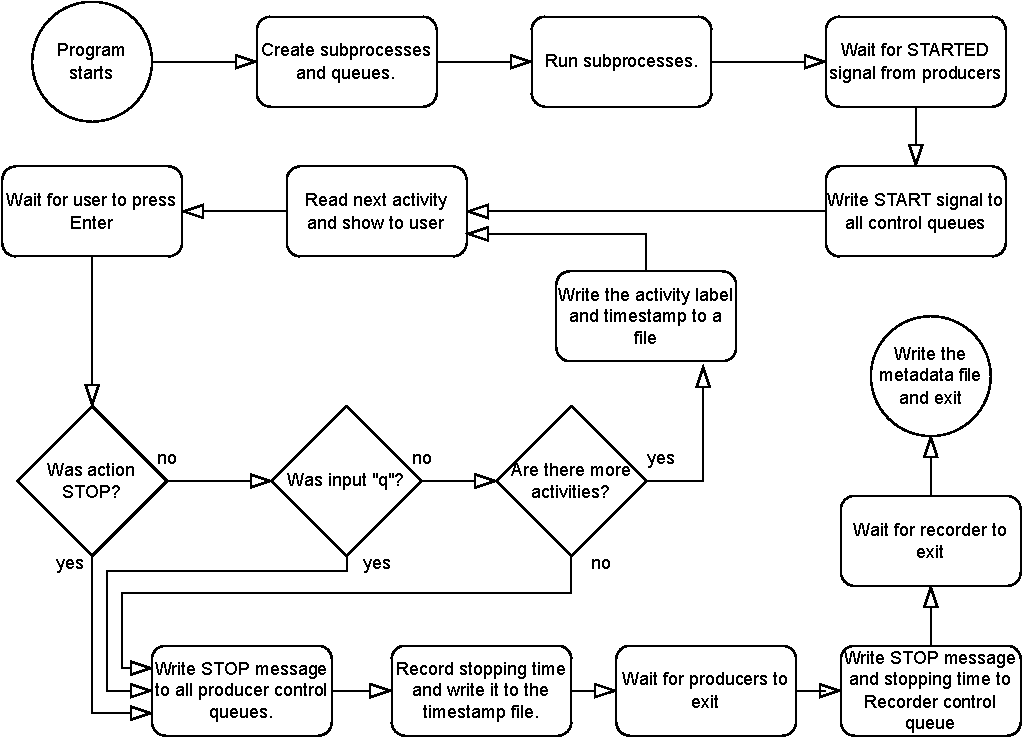
\includegraphics[width=0.9\textwidth]{fig/3/main-flowchart.pdf}
    \caption{Flow of the main process}
    \label{fig:3-main-flowchart}
\end{figure}

The following Sections (\ref{sec:3-recorder}--\ref{sec:3-mic}) will document the implementation of the subprocesses.
For the data producers, communication with the sensors will be documented, and for the Recorder,
the time-domain synchronization mechanism will be documented.
The three phases of operation will be described similar to the former description of the Main process.
Section \ref{sec:3-usage} will briefly cover usage of the software.

\section{Recorder block}
\label{sec:3-recorder}
The Recorder module is the only consumer in the program.
It takes the data produced by the producers and writes it into a file.
It is also responsible for time-domain synchronization of the different data streams.

The initialization phase of the Recorder block consists of opening file handles for the output files and initializing some counters.
In the beginning of the second phase, i.e. after receiving the START message,
the Radar block finds the common starting point for each data producer and synchronizes the data streams to the common starting point.
After the data streams are synchronized, the Recorder enters a loop in which it simply reads the data from each data queue and writes it onto a disk.

Time synchronization is achieved in the Recorder block by observing the time stamps that the producers add to the packets they write in data queues.
Each packet is a dict object that contains a segment of data and the time stamp when the data segment was recorded.

By the time the START message is received from the control queue,
all the data producers have started producing data and have written their first message to the data queues.
After the START message, the Main process also writes the current time to the control queue of the Radar block.
The common starting point is found by comparing the time stamps in the data queues to the starting time provided by the Radar block.
The data in each data queue is simply discarded until the timestamp is within half-a-frame from the starting time.
After the appropriate amount of data has been discarded from each queue,
the data streams are synchronized and the Recorder starts writing the data into files.
The data starting point synchronization procedure is presented in pseudocode in Listing \ref{lst:synchronization}.
The half-a-frame accuracy is omitted from the listing for brevity.

\begin{lstlisting}[language=Python, caption={Data synchronization pseudocode}\label{lst:synchronization}]
while control_queue.pop() != "START":
    pass
start_time = control_queue.pop()

for queue in data_queues:
    message = queue.pop()
    timestamp = message["timestamp"]
    data = message["data"]
    
    while (timestamp < start_time):
        message = queue.pop()
        timestamp = message["timestamp"]
        data = message["data"]
\end{lstlisting}

Finally, when the user stops the system, the Main process sends the STOP message to the Recorder control queue,
and in succession, the stopping time .
By this time, the data producers have already exitted and no more data will be written to the output queues.
The Recorder then enters the last phase of operation,
which is the stream end synchronization.

The stopping time is recorded before the STOP signal is sent to the data producers.
Knowing this, finding the common ending point is trivial,
and the algorithm presented in Listing \ref{lst:synchronization} can be modified for the purpose.
Instead of the starting time, the time stamps are compared to the ending time,
and instead of discarding the data, it is written into a file.
The modified algorithm is presented in Listing \ref{lst:end-synchronization}.

\begin{lstlisting}[language=Python, caption={Data synchronization pseudocode}\label{lst:end-synchronization}]
while (control_queue.empty() or control_queue.pop() != "STOP"):
    for queue in data_queues:
        message = queue.pop()
        data = message["data"]
        # write data to file
        
end_time = control_queue.pop()

for queue in data_queues:
    message = queue.pop()
    timestamp = message["timestamp"]
    data = message["data"]
    
    while (timestamp < end_time):
        message = queue.pop()
        timestamp = message["timestamp"]
        data = message["data"]
        # write data to file
\end{lstlisting}

After the end synchronization procedure is finished,
the Recorder will flush the data queues discarding all remaining data,
and close the file handles.
After freeing the resources and flushing the queues, the process will exit.

\section{Radar block}
\label{sec:3-radar}
The radar module actually consists of two devices: the Texas Instruments IWR6834ISK and the DCA1000EVM Radar Data capture card.
In this section, the former is referred to as the "radar device" and the latter as the "capture card".
The radar device connects to the computer via USB and implements a simple serial interface.
The capture card uses Internet Protocol version 4 to connect to the computer and transfers data over the User Datagram Protocol.

In the Radar block, the Pyserial third-party library is used to connect to the serial interface.
The Pyserial library implements an easy-to-use high-level serial port \gls{api}. \cite{python-serial}
The serial port was configured to use a baud rate of 115200 bps and no parity.

For reading data from the capture card, the built-in Socket library is used.
The Socket library implements the Berkeley Socket interface.
By default, the capture card is listening at address \texttt{192.168.33.180:4096} and sends data to address \texttt{192.168.33.30:4098}.
The addresses could be configured differently, but it was deemed easier to just configure an extra \gls{ipv4} address to the host computer. \cite{dca1000-user-guide}

In the initialization phase, the Radar block configures the radar device and the capture card.
Configuring the radar device is done by writing a special configuration file to the serial interface.
The exact format of the configuration file is documented in the Texas Instruments mmWave SDK user guide \cite{mmwave-sdk-user-guide}.
The configuration file used during the testing and development of this system is included as Appendix \ref{app:config}.

The capture card is configured by transmitting special configuration packets to the address it is listening to.
The packets consist of a header (\texttt{0x055A}), a two-byte unsigned integer length field, command identifier, body, and a footer (\texttt{0xEEAA}).
The commands are listed in the DCA1000EVM user guide \cite{dca1000-user-guide} and the details of the command bodies are documented in 
DCA1000EVM CLI Software Developer guide, which is included in the Texas Instruments mmWave studio collection of tools \cite{mmwave-studio}.
For the sake of availability, the commands and their bodies are also documented in Appendix \ref{app:dca1000evm-commands}.
While most settings are left to default values, the LVDS mode is changed to 2lane and Data format mode is changed to 16-bit.
This is done via the CONFIG\_FPGA\_GEN\_CMD\_CODE command (Appendix \ref{app:dca1000evm-commands}, Section \ref{app:sec:config-fpga}).

After configuration is done, the devices must also be started.
The radar device can be started by writing "\texttt{sensorStart\textbackslash n}" to the serial interface.
The capture card is started by sending the RECORD\_START\_CMD\_CODE (Appendix \ref{app:dca1000evm-commands}, Section \ref{app:sec:start-record}).
The capture card should then respond with status 0, indicating that the recording has been successfully started,
thus concluding the initialization phase.

After starting the radar device and the capture card,
the Radar module writes the STARTED message to the control queue and begins its primary function phase.
In the primary function,
the Radar module listens to the socket \texttt{192.168.33.30:4098} and reads data from it whenever available.

The Radar process can read the number of samples per frame from the radar configuration file.
With this information, it is possible to organize the received data into frames and write them into the data queue frame-by-frame.
The inter-frame time is also known from the configuration file.
The radar device or the capture card do not add any timing information to the outputted data.
The Radar process therefore records the current time when the first byte of the first frame is received, i.e. the starting time.
The starting time is then used to calculate time stamps for the frames.
For each received frame, a counter is incremented. The time offset of the frame is calculated from the counter and the inter-frame time and added to the starting time
to form the time stamp for the frame.

The process simply reads data from the socket to a buffer until the buffer contains a single frame.
When enough data is in the buffer, a dict-object containing the data of the frame and a time stamp for the frame is written into the data queue.
The frame is then deleted from the beginning of the buffer and the loop is continued until the STOP message is received.
The flow of the Radar module is represented as a flow chart in Figure \ref{fig:3-radar-flowchart}.

\begin{figure}[H]
    \centering
    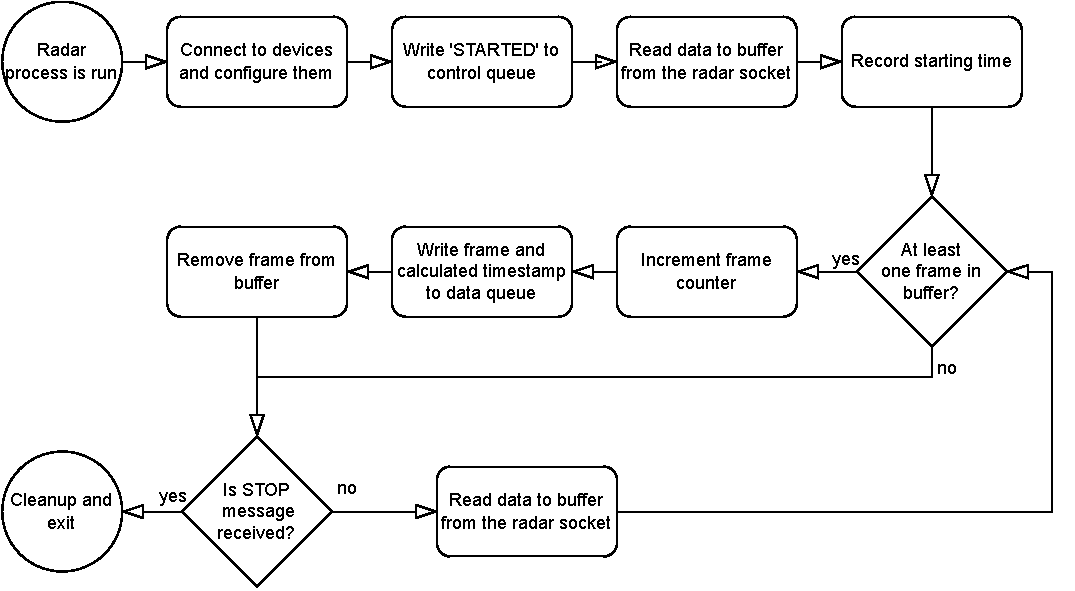
\includegraphics[width=\textwidth]{fig/3/radar-flowchart.pdf}
    \caption{Flow of the Radar module}
    \label{fig:3-radar-flowchart}
\end{figure}

After the STOP message is received,
all the sockets and serial connections are closed.
Additionally, the remaining data from the buffer is discarded and the data queue is closed from being written to.
Thus, the clean up is concluded and the Radar process exits.

\section{RGB-D block}
\label{sec:3-rgb-d}
Intel provides the Librealsense library for working with the camera with multiple programming languages.
For this implementation, the Pyrealsense2 library was used, which implements Python bindings for the Librealsense library. \cite{librealsense2}
The Librealsense provides a high-level \gls{api} for configuring the device and reading data from it.
Configuring is done via a \texttt{Config} object and reading data is done via a \texttt{Pipeline} object. \cite{librealsense2-python-docs}

In the initialization phase of the RGB-D process, the \texttt{Config} and \texttt{Pipeline} objects are created.
The used data streams must be explicitly enabled via the \texttt{Config} object.
The depth and color streams are enabled.
The functions that enable the streams also configure the frame rate, resolution, and number format for the data.
In this implementation, the resolutions and frame rates are read from a configuration file provided by the user.
The colored stream is configured to output data in the RGB8 format, where each pixel is represented by three bytes.
The bytes are one-byte unsigned integers. The first byte is the red value, second byte is the green value and third byte is the blue value.
The depth stream is configured to output data as 2-byte floating point numbers,
where each pixel, or a 2-byte floating point number, represents the distance from the camera in the direction of the pixel.

After configuring the data streams, the \texttt{Pipeline} object is used to start the sensor.
After the sensor has been started, the process writes the STARTED message to the control queue and enters its primary function.

In the primary function, the process reads frames from the \texttt{Pipeline} object using a member function of the Pipeline object that blocks until a frame is available.
The function call returns a \texttt{composite\_frame} object that contains the stream data, a time stamp, and some other less interesting metadata.
The RGB-D process reads the color stream data and the depth stream data into arrays and stores them in a \texttt{dict} object along the time stamp for the frame,
which is also read from the \texttt{composite\_frame}.
The \texttt{dict} object is then written into the data queue and the process is repeated until the STOP message is received from the control queue.

When the STOP message is received,
the RGB-D process transitions into its cleanup phase.
In the cleanup phase, the process simply exits,
which calls the destructors of the Pyrealsense2 objects,
which in turn stop the sensors and free their allocated resources.
Figure \ref{fig:3-rgbd-flowchart} illustrates the flow of the RGB-D process.

\begin{figure}
    \centering
    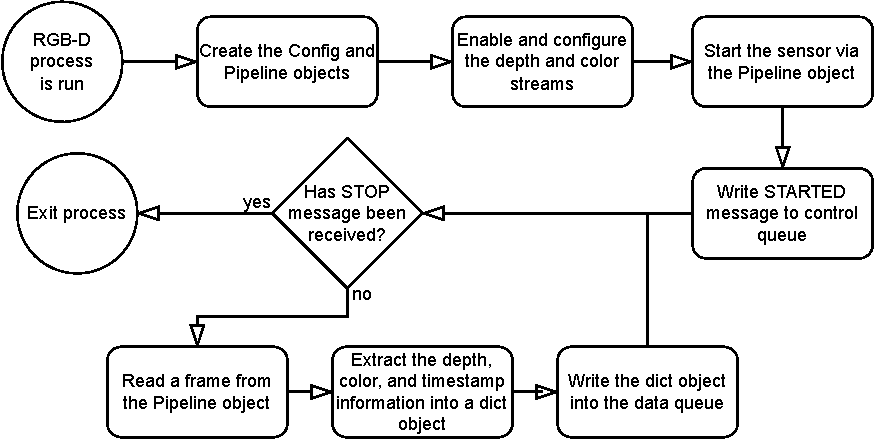
\includegraphics{fig/3/rgbd-flowchart.pdf}
    \caption{Flow of the RGB-D process}
    \label{fig:3-rgbd-flowchart}
\end{figure}

\section{Infrared block}
\label{sec:3-ir}
Similar to the TI IWR6843ISK, the Panasonic GRID-EYE implements a simple serial interface over USB.
Pyserial was also used for connecting to the GRID-EYE.
Two kinds of packets are implemented for the GRID-EYE protocol: Sensor Data frames and Command frames.
The Command frames are used by the connecting computer to configure the device and after being started,
the device will write Sensor Data frames to the serial port.
The Command frames can be used to set the sensor into either 10 \gls{fps} for 1 \gls{fps} mode. \cite{grid-eye-protocol}
The sensor is used in the 10 \gls{fps} mode in the system, because the 1 \gls{fps} mode is only the sum of every 10 frames
and similar effect can easily be achieved by post-processing the data after recording \cite{grid-eye-manual}.

In the initialization phase, the IR process opens the serial port (9600 bps, no parity, one stop bit, 8-bit byte size).
The device requires no further configuration as it operates in the 10 \gls{fps} mode by default.
After opening the serial port, the data in the serial port is flushed,
and the STARTED message is written to the control queue,
concluding the initialization phase.

After the initialization phase, the process immediately begins the primary function.
In the primary function, the process reads data from the serial port in 135-byte chunks.
The 5th--132th (0-indexing) bytes contain the temperatures for each of the pixels as two-byte little-endian integers.
Every two bytes is a multiple of four of the temperature reading.

The Python built-in Struct library is used to unpack the raw data to numeric values.
Conveniently, two-byte floating point numbers can accurately represent integer multiples of $0.25$.
Using this knowledge, the unpacked numbers are divided by four and repacked as two-byte floating point numbers.
The repacked floating point numbers are then stored in a \texttt{dict} object with a time stamp that is sourced 
from the computer clock using the \texttt{perf\_counter} function from the Python built-in Time library.
The process is then repeated until the STOP message is received from the control queue.

After receiving the STOP signal, the clean-up phase begins.
In the clean up, the process simply exits,
which frees the serial port file handle.
No other resources were allocated in the process.
The flow of the system is illustrated in Figure \ref{fig:3-ir-flowchart}.

\begin{figure}
    \centering
    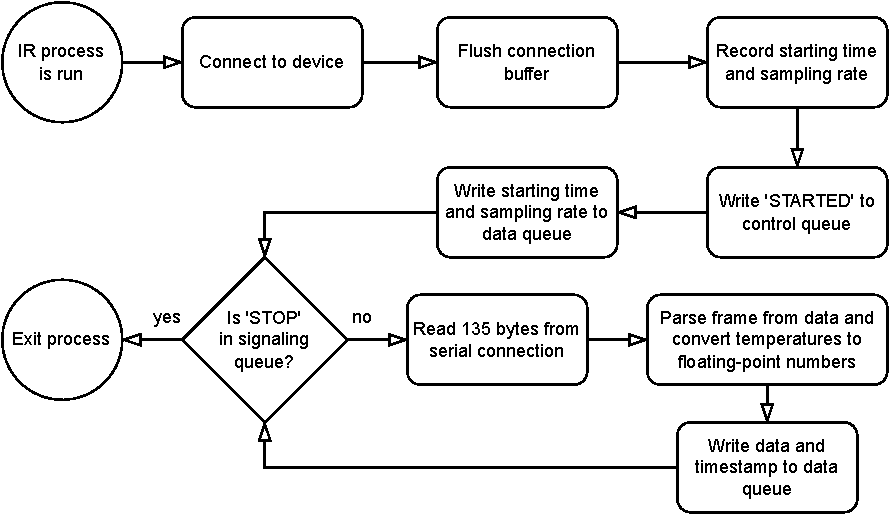
\includegraphics[width=\textwidth]{fig/3/ir-flowchart.pdf}
    \caption{Flow of the IR process}
    \label{fig:3-ir-flowchart}
\end{figure}

\section{Microphone block}
\label{sec:3-mic}
Unlike the other devices, the data produced by the microphone cannot be organized into frames.
It produces a continuous stream of data on all 16 channels at a configurable sampling rate and bit depth.
The SoundDevice library is used for interfacing with the device \cite{sounddevice-docs}.
It provides Python bindings for the PortAudio library,
which, among other features, has the ability to pick a sound device,
configure it to a wished sampling rate and bit depth, and record audio from it \cite{portaudio}.

Picking a device is done via the \texttt{query\_devices} function,
which returns information about available devices.
It accepts two arguments.
The first argument is a numeric device ID or the name of the device as a string.
If the first argument is given, only the information of one device is returned.
The second parameter can be used to list only input or output devices. \cite{sounddevice-docs}.

The SoundDevice library implements an \gls{api}, where \texttt{Stream} objects are created and attached to audio devices.
The \texttt{Stream} objects can then write to and read from devices.
A callback function may be passed to the constructor of the \texttt{Stream} object,
which is periodically called automatically by the PortAudio library.
The callback function handles writing data to the device and provides access to the read data. \cite{sounddevice-docs-stream}

The callback function may also be omitted,
in which case reading and writing should be done via the blocking \texttt{read} and \texttt{write} functions.
Using the callback function is the preferred way of using the interface,
as the callback function automatically has a high processing priority.
To achieve robust audio with minimal latency, 
the callback function should not call functions with long or unpredictable execution times. \cite{sounddevice-docs-stream}

After the \texttt{Stream} object has been instantiated,
the stream must also be started.
This can be done via \texttt{start} and \texttt{stop} functions.
The stream objects are also context managers and when used in the \texttt{with}-statement,
the \texttt{start} and \texttt{stop} functions are automatically called in the beginning and end of the statement, respectively. \cite{sounddevice-docs-stream}
Context managers and the \texttt{with} statement are a part of the Python programming language.

The initialization phase of the Microphone module finds the correct sound device and constructs and \texttt{InputStream} context manager,
which is a specialized \texttt{Stream} object that can only be used for input devices.
Searching the device is done via the \texttt{query\_devices} function with the first argument set to "micArray16".
The device is then set as the default device in the SoundDevice library.
Upon instantiation, the \texttt{InputStream} object will utilize the default device without further configuration.

The configuration is done in the constructor of the \texttt{InputStream} object.
The sampling rate is set to 44.1 kHz, bit depth to 32 bits and recording is done on all 16 channels of the device.
After instantiating the \texttt{InputStream} object, the STARTED signal is written to the control queue and the primary function is entered, ending the initialization phase.

The primary function is a simple busy-loop that observes the control queue.
The process runs until the STOP message is read from the control queue.
While waiting for the STOP message,
the callback function is being periodically called by the PortAudio library.
The callback function writes data from the device to the data queue along the timestamp for when the callback was called.
The timestamp is derived using the \texttt{perf\_counter} function from the built-in Time library.

\begin{figure}[H]
    \centering
    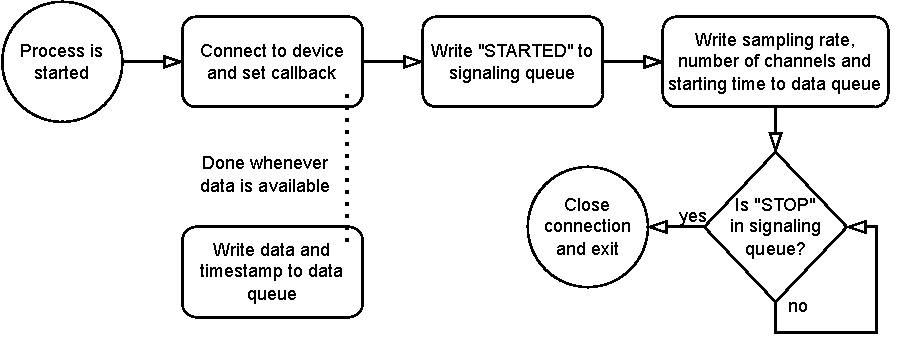
\includegraphics[width=\textwidth]{fig/3/mic-flowchart.pdf}
    \caption{Flow of the Microphone block}
    \label{fig:mic-flowchart}
\end{figure}

When the STOP message is received from the control queue,
the aforementioned busy-loop exits, ending the \texttt{with}-statement and stopping the \texttt{InputStream} instance.
The Microphone process then exits.
The logic of the Microphone process is presented as a flowchart in Figure \ref{fig:mic-flowchart}.

\section{Using the software}
\label{sec:3-usage}
The software is started via a \gls{cli} that is implemented using the Python built-in \texttt{argparse} library.
Three positional arguments must be provided for the program: \texttt{activities}, \texttt{config}, and \texttt{outdir}.
All of the arguments are file paths.

The first argument, \texttt{activities}, can be used to provide a list of activities for the software.
This can be used for semi-automatic activity labelling during the recording process.
This is useful when recording a predetermined list of activities.
The activities must be separated by newline (\texttt{\textbackslash n}) characters.
The software outputs a \gls{csv} file which contains the same list of activities,
but each activity is assigned a timestamp.
The file can also be empty, in which case no timestamps will be recorded other than the starting and stopping time.

The second argument, \texttt{config}, is a configuration file for the program.
The values present in the file are used to configure the sensors.
The file must follow the YAML data serialization language.
An example file is provided in Listing \ref{lst:config}.

\begin{lstlisting}[caption={Example configuration file}\label{lst:config}]
radar:
    config: filename
camera:
    resolution: [width, height]
    fps: integer
\end{lstlisting}

Under the key \texttt{radar}, the \texttt{filename} that is the value of \texttt{config} must refer to a configuration file for the TI IWR6843ISK radar device.
Under the key \texttt{camera}, the value of \texttt{resolution} must be a two-element list whose values are some supported resolution of the Intel RealSense 435i camera.
Similarly, the \texttt{fps} must be some supported frame rate of the camera.
The values under the key \texttt{camera} are used for both the RGB and Depth stream.
The \gls{ir} and microphone devices should preferrably be configured via the same file but due to time constraints,
they were left hardcoded.

The last argument, \texttt{outdir}, must be a directory path.
The files created by the software are written into this directory.
The output files and their exact formats are documented in Chapter \ref{ch:4-files-and-post}.
